\documentclass[a4paper,12pt]{article} % тип документа

% report, book

%  Русский язык
\usepackage{multirow}
\usepackage{wrapfig}
\usepackage[T2A]{fontenc}			% кодировка
\usepackage[utf8]{inputenc}			% кодировка исходного текста
\usepackage[english,russian]{babel}	% локализация и переносы

\usepackage{indentfirst} %Красная строка
\usepackage[a4paper,top=1.3cm,bottom=2cm,left=1.5cm,right=1.5cm,marginparwidth=0.75cm]{geometry}
\usepackage[usenames]{color}
\usepackage{colortbl}

% Заметки
\usepackage{todonotes}

% Математика
\usepackage{amsmath,amsfonts,amssymb,amsthm,mathtools} 
\usepackage{hyperref}

\begin{document}

\begin{titlepage}
\begin{center}
    {\large МОСКОВСКИЙ ФИЗИКО-ТЕХНИЧЕСКИЙ ИНСТИТУТ (НАЦИОНАЛЬНЫЙ ИССЛЕДОВАТЕЛЬСКИЙ УНИВЕРСИТЕТ)}
\end{center}
\begin{center}
    {\largeФизтех-школа биологической и медицинской физики}
\end{center}


    \vspace{3.5cm}

\begin{center}
    
\includegraphics[width=0.4\linewidth]{hv_full.png}
\end{center}
\vspace{0.1cm}
{\huge
\begin{center}
    {\bf Лабораторная работа 2.2(2.3)}\\
    Изучение спектров атома водорода и молекулы йода
\end{center}
}
\vspace{2cm}
\begin{flushright}
{\LARGE Авторы:\\ Ирина Веретененко \\
\vspace{0.2cm}
Б06-804}
\end{flushright}
\vspace{3.5cm}
\begin{center}
    Долгопрудный 2020
\end{center}
\end{titlepage}

\section*{Введение}

\textbf{Цель работы}: 
\begin{enumerate}
    \item Провести калибровку барабана спектрометра по спектрам неона и ртути
    \item Определить длины волн нескольких первых спектральных линий серии Бальмера для водорода, рассчитать постоянную Ридберга
    \item Определить длины волн нескольких первых спектральных линий нулевой серии Деландера молекулы йода, вычислить энергию колебательного кванта, энергию диссоциации в основном и возбужденном состоянии 
\end{enumerate}

\textbf{В работе используются}: Стеклянно-призменный монохроматор-спектрофотометр УМ-2, водородная лампа, лампа накаливания, кристаллы йода




\subsection*{Теория}
\subsubsection*{A.Изучение спектра атома водорода}
\begin{wrapfigure}[19]{R}{0.4\linewidth} 
\center{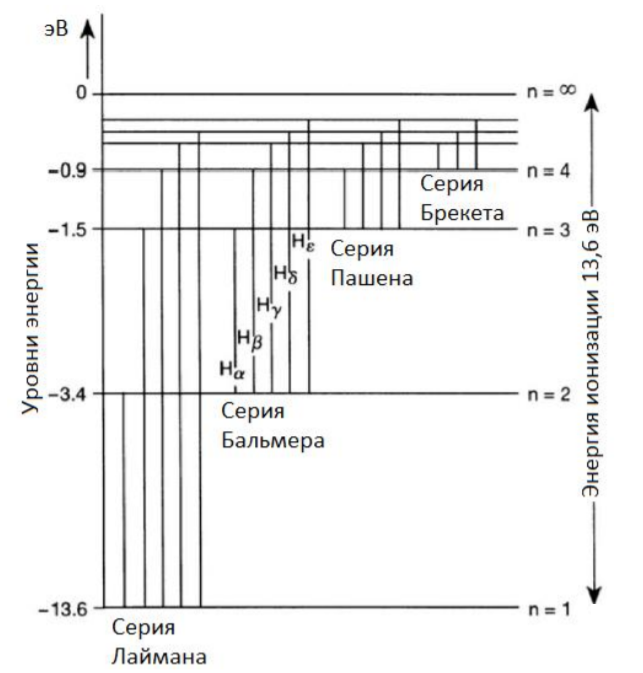
\includegraphics[scale=0.5]{спектр водорода2.jpg}}
\caption{Уровни энергии атома водорода. Спектральные серии}
\label{fig:image}
\end{wrapfigure}

Атомный спектр - это спектр, получающийся при испускании/поглощении света свободным атомом. \\


Обобщенная формула Бальмера (получена экспериментально):
\begin{equation}
    \frac{1}{\lambda_{mn}} = RZ^2(\frac{1}{n^2} - \frac{1}{m^2})
\end{equation} где
\begin{itemize}
    \item $\lambda_{mn}$ - длина волны, на которой может поглощать/излучать водородоподобный атом
    \item $R = 109677,6 \text{см}^{-1}$ - постоянная Ридберга
    \item $Z$ - заряд ядра атома
    \item $n, m \in Z$
\end{itemize}

Энергетические состояния электрона в атоме водорода (получены из постулатов Бора):
\begin{equation}
    E_n = -\frac{2\pi^2m_e e^4 Z^2 }{h^2}\frac{1}{n^2}
\end{equation}

В данной работе изучается серия Бальмера ($n = 2$), линии которой лежат в видимой области. Первые 4 линии этой серии обозначаются $H_\alpha, H_\beta, H_\gamma, H_\delta$. Для них $m = 3, 4, 5, 6$ соответственно. .

\subsubsection*{B. Изучение молекулярного спектра йода}
Энергия молекулы (считая, что возбуждения независимы):
\begin{equation*}
    E \approx E_{\text{эл}} + E_{\text{колеб}} + E_{\text{вращ}}
\end{equation*}
\begin{enumerate}
    \item Электронные уровни молекулы (стационарные состояния) аналогичны уровням энергии изолированных атомов
    
    \item Колебательные возбуждения возникают при смещении атомов в молекуле от равновесных положений. Энергия колебаний атомов молекулы на электронном уровне $E = \hbar \omega_0$: 
    \begin{equation*}
        E_{\text{колеб}} = \hbar \omega_0 (n + \frac{1}{2}) - \hbar \omega_0 x_n (n + \frac{1}{2})^2
    \end{equation*}
    Первое слагаемое - энергия гармонического осциллятора с частотой $w_0$ ($n$ - колебательное квантовое число), второе - отступление от гармонического закона ($x_n$ - коэффициент агармонизма).\\ На рис.2 слева показан график потенциальной энергии в зависимости от расстояния между ядрами для 2атомной молекулы на фиксированном электронном уровне. На малых расстояниях кривая - парабола, нижние уровни энергии близки к уровням гармонического осциллятора, поэтому при малых n вторым слагаемым можно пренебречь. Но при увеличении расстояния агармоничность начинает давать все больший вклад, потенциальная энергия стремится к постоянному значению. В этот момент происходит \textbf{диссоциация молекулы}. Энергия диссоциации обозначена $D$. Выше энергии диссоциации мы видим непрерывный спектр. 
    
    \item Вращательные возбуждения - дискретные состояния, соответствующие вращению молекулы как целого вокруг некоторой оси. 
\end{enumerate}
 \textbf{Оптические переходы} (переходы, связанные с излучением фотонов в видимом диапазоне длин волн) соответствуют переходом между различными электронными состояниями. При этом происходят изменения вращательного и колебательного состояний. \\\\
 В данной работе будет исследоваться спектр поглощения паров йода ($I_2$) в видимой области. \\ 
 Можно оценить, что для двухатомной молекулы 
 \begin{equation*}
     \omega_{\text{эл}} : \omega_{\text{колеб}} : \omega_{\text{вращ}} = 1 : 10^{-3} : 10^{-6}
 \end{equation*}
 Так как энергия вращательных движений в $10^{6}$ раз меньше электронной, то в видимой области наблюдаются только электронно-колебательные спектры молекул.

 \begin{figure}[h!]
\center{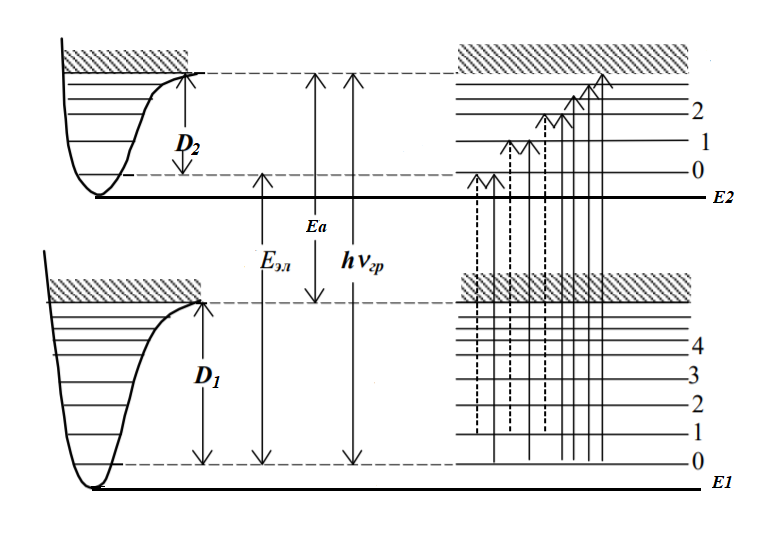
\includegraphics[scale=0.7]{ceg.png}}
\caption{Структура электронно-колебательного спектра поглощения молекулы йода в видимой области. $E_1$ - основное состояние, $E_2$ - возбужденное. Тонкие горизонтальные линии - колебательные уровни энергии для данных состояний. Косые штрихи - области непрервыного спектра}
\label{fig:image}
\end{figure}


\textbf{Серии Деландера} - это серии переходов между соседними электронными состояниями, соответствуюющие одному начальному колебательному состоянию. \\
Можно оценить, что самой интенсивной будет 0 серия, а серии больше 3-й наблюдаться практически не будут (т.к. на исходном колебательном уровне не будет достаточного числа электронов)\\

 
\subsection*{Экспериментальная установка}
\subsubsection*{А. Изучение спектра атома водорода}
\begin{wrapfigure}[12]{r}{0.5\linewidth} 
\vspace{-5ex}
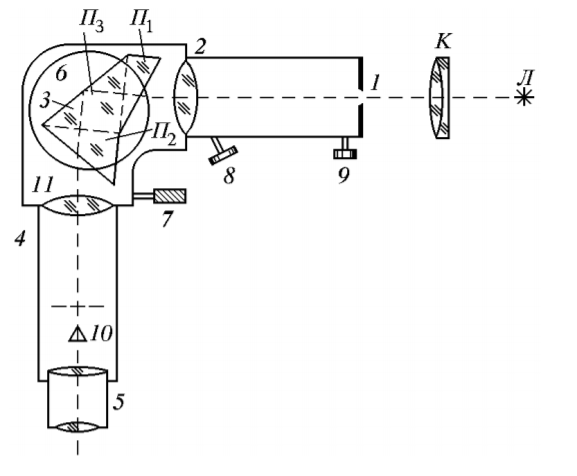
\includegraphics[width=\linewidth]{установка водород.png}
\caption{Стеклянно-призменный монохроматор-спектрометр УМ-2, диапазон измеряемых длин волн 0.38-1 мкм}
\label{fig:somelabel}
\end{wrapfigure}

Основные элементы спектрометра: 
\begin{itemize}
    \item Входная щель 1
    \item Колиматорный объектив 2
    \item Сложная спектральная призма 3, состоящая из склееных призм П$_1$, П$_2$, П$_3$
    \item Зрительная труба: объектив 4 и окуляр 5
    \item Поворотный столик 6
    \item Микрометрические винты 7-9
    \item Острие указателя 10
    \item Массивный корпус 11
\end{itemize}
Источник света - водородная трубка

\subsubsection*{B. Изучение молекулярного спектра йода}
\begin{wrapfigure}[8]{r}{0.5\linewidth} 
\vspace{-5ex}
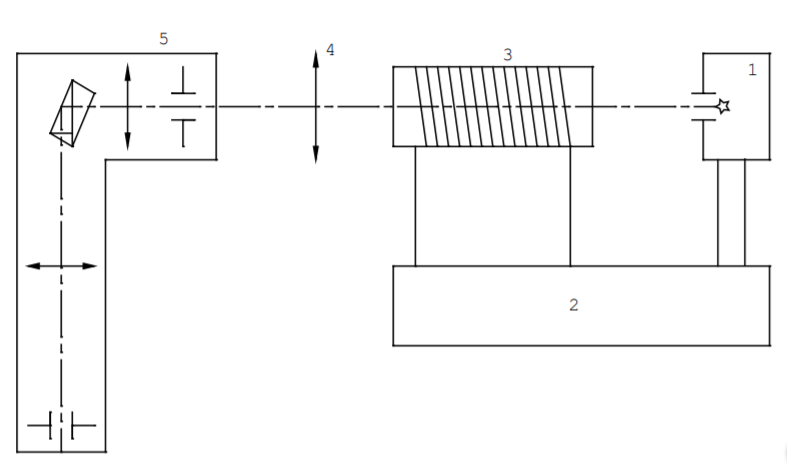
\includegraphics[width=\linewidth]{установка йод.png}
\caption{Установка для измерения спектра поглощения йода}
\label{fig:somelabel}
\end{wrapfigure}
Основные элементы установки:
\begin{itemize}
    \item Лампа накаливания 1- источник сплошного спектра
    \item Блок питания 2
    \item Кювета с исследуемым веществом 3- поглощающая среда
    \item Линза 4
    \item Монохроматор УМ-2 5
\end{itemize}

\newpage
\section*{Ход работы и обработка результатов}
\subsection*{Калибровка барабана спектрофотометра}
Проградуируем спектрофотометр по известным спектрам неона и ртути. По результатам измерений построим калибровочный график, переводящий показания барабана спектрофотометра, настроенного на спектральную линию,  в соответствующую этой линии длину волны.
\\

\begin{wrapfigure}[0]{r}{0.6\linewidth} 
\vspace{-40ex}
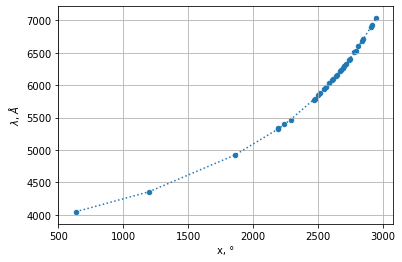
\includegraphics[width=\linewidth]{калибр.png}
\caption{ \centering калибровочный график\\ Уравнение калибровочной кривой:
\begin{equation*}
    \lambda, A  =  a_4 \cdot x^4 + a_3 \cdot x^3 + a_2  \cdot x^2  a_1 \cdot x + a_0\\
    a_4 = 1.225 \cdot 10^{-10}, a_3 = -6.545 \cdot 10^{-7}, a_2 = 1.511 \cdot 10^{-3}, \\ a_1 = - 9.335 \cdot 10^{-1}, a_0 = 4.179\cdot 10^{3}
\end{equation*}}
\label{fig:somelabel}
\end{wrapfigure}


\begin{floatingtable}
\begin{tabular}{|c|c|cc}
\hline
\multicolumn{2}{|c|}{неон} & \multicolumn{2}{c|}{ртуть} \\ \hline
$\lambda$, A & $x^{\circ}$ & \multicolumn{1}{c|}{$\lambda$, A} & \multicolumn{1}{c|}{$x^{\circ}$} \\ \hline
7032 & 2944 & \multicolumn{1}{c|}{6907} & \multicolumn{1}{c|}{2910} \\ \hline
6929 & 2914 & \multicolumn{1}{c|}{6234} & \multicolumn{1}{c|}{2672} \\ \hline
6717 & 2848 & \multicolumn{1}{c|}{5791} & \multicolumn{1}{c|}{2478} \\ \hline
6678 & 2836 & \multicolumn{1}{c|}{5770} & \multicolumn{1}{c|}{2468} \\ \hline
6599 & 2808 & \multicolumn{1}{c|}{5461} & \multicolumn{1}{c|}{2290} \\ \hline
6533 & 2788 & \multicolumn{1}{c|}{4916} & \multicolumn{1}{c|}{1862} \\ \hline
6507 & 2776 & \multicolumn{1}{c|}{4358} & \multicolumn{1}{c|}{1198} \\ \hline
6402 & 2744 & \multicolumn{1}{c|}{4047} & \multicolumn{1}{c|}{634} \\ \hline
6383 & 2734 & \multicolumn{2}{c}{\multirow{17}{*}{}} \\ \cline{1-2}
6334 & 2714 & \multicolumn{2}{c}{} \\ \cline{1-2}
6305 & 2700 & \multicolumn{2}{c}{} \\ \cline{1-2}
6267 & 2688 & \multicolumn{2}{c}{} \\ \cline{1-2}
6217 & 2666 & \multicolumn{2}{c}{} \\ \cline{1-2}
6164 & 2644 & \multicolumn{2}{c}{} \\ \cline{1-2}
6143 & 2634 & \multicolumn{2}{c}{} \\ \cline{1-2}
6096 & 2616 & \multicolumn{2}{c}{} \\ \cline{1-2}
6074 & 2606 & \multicolumn{2}{c}{} \\ \cline{1-2}
6030 & 2584 & \multicolumn{2}{c}{} \\ \cline{1-2}
5976 & 2562 & \multicolumn{2}{c}{} \\ \cline{1-2}
5945 & 2548 & \multicolumn{2}{c}{} \\ \cline{1-2}
5882 & 2512 & \multicolumn{2}{c}{} \\ \cline{1-2}
5852 & 2502 & \multicolumn{2}{c}{} \\ \cline{1-2}
5401 & 2238 & \multicolumn{2}{c}{} \\ \cline{1-2}
5341 & 2194 & \multicolumn{2}{c}{} \\ \cline{1-2}
5331 & 2190 & \multicolumn{2}{c}{} \\ \cline{1-2}
\end{tabular}
\end{floatingtable}

\subsection*{Спектр атома водорода}
\begin{itemize}
    \item Измерим положение линий спектра атома водорода $H_\alpha, H_\beta, H_\gamma$ (последняя линия $H_\delta$ не видна). 
    \item Из уравнения калибровочной кривой найдем соответствующие линиям спектра длины волн. \\
Формулы для расчета ($\sigma x = 10^{\circ}$ - цена деления барабана 2 + неточности наведения прибора на нужную длину волны):
\begin{equation*}
    \lambda, A  =  a_4 \cdot x^4 + a_3 \cdot x^3 + a_2  \cdot x^2  a_1 \cdot x + a_0 
\end{equation*}
\begin{equation*}
    \sigma \lambda = (a_1 + a_2 \cdot x + a_3 \cdot x^2 + a_4 \cdot x^3) \cdot \sigma x
\end{equation*}
Также рассчитаем для каждой длины волны ее теоретическое значение
\begin{equation*}
    \lambda = \frac{1}{R(\frac{1}{n^2} - \frac{1}{m^2})}, R_{\text{теор}} = 109677.6\text{см}^{-1}
\end{equation*}
\item Для каждой линии расчитаем постоянную Ридберга и найдем среднее значение.\\ Формулы для расчета ($n = 2$, $m = 3, 4, 5$, заряд ядра водорода $Z = 1$):
\begin{equation*}
    R = \frac{1}{\lambda_{nm} \cdot (\frac{1}{n^2} - \frac{1}{m^2})}, \sigma R = \frac{\sigma \lambda_{nm}}{\lambda^2 \cdot (\frac{1}{n^2} - \frac{1}{m^2})}
\end{equation*}
\begin{equation*}
    \bar R = \frac{\sum R_i}{3}, \sigma \bar R = \sqrt{\frac{1}{3\cdot 2} \sum (R_i - \bar R)^2}
\end{equation*}

\begin{table}[h!]
\centering
\begin{tabular}{|c|c|c|c|c|c|c|c|c|}
\hline
 & $x^{\circ}$ & $\lambda, A$& $\sigma \lambda, A$ & $n$ & $m$ & $R$, см$^{-1}$ & $\sigma R$, см$^{-1}$ & $\lambda_\text{теор}, A$ \\ \hline
$H_\alpha$ & 2814 & 6610 & 30 & 2 & 3 & 108900 & 500 & 6565 \\ \hline
$H_\beta$ & 1802 & 4860 & 10 & 2 & 4 & 109600 & 200 & 4863
\\ \hline
$H_\gamma$ & 1162 & 4331 & 7 & 2 & 5 & 109900 &  200 & 4342 \\ \hline
\end{tabular}
\end{table}
 


Экспериментальное значение постоянной Ридберга.

\begin{equation*}
\boxed{
    \bar R = (109500 \pm 300) \text{см}^{-1}}
\end{equation*} 
Полученное значение  хорошо согласуется с теоретическим $R_{\text{теор}} = 109677.6 \text{см}^{-1}$

\item

Проверим, что отношение длин волн соответствует формуле сериальной закономерности (в принципе, это видно из того, что каждая из длин волн соответствует своему теоретическому значению в пределах погрешности)\\
\begin{equation*}
    \frac{1}{\lambda_{nm}} \sim (\frac{1}{n^2} - \frac{1}{m^2})
 \xRightarrow{}  \frac{\lambda_{nm_1}}{\lambda_{nm_2}} = \frac{\frac{1}{n^2} - \frac{1}{m_2^2}}{\frac{1}{n^2} - \frac{1}{m_1^2}}
\end{equation*}

\begin{equation*}
    \sigma(\frac{\lambda_1}{\lambda_2} )= \frac{\lambda_1}{\lambda_2} \sqrt{(\frac{\sigma \lambda_1}{\lambda_1})^2 + (\frac{\sigma \lambda_2}{\lambda_2})^2}
\end{equation*}
\begin{equation*}
    \frac{\frac{1}{2^2} - \frac{1}{4^2}}{\frac{1}{2^2} - \frac{1}{3^2}} = 1.35, \frac{\lambda_\alpha}{\lambda_\beta} = 1.36 \pm 0.01
\end{equation*}
\begin{equation*}
    \frac{\frac{1}{2^2} - \frac{1}{5^2}}{\frac{1}{2^2} - \frac{1}{4^2}} = 1.12, \frac{\lambda_\beta}{\lambda_\gamma} = 1.12 \pm 0.01
\end{equation*}
\end{itemize}




\subsection*{Спектр паров йода}
\begin{itemize}
    \item На установке получим спектр йода. 
    Примерный вид спектра: 
    \begin{figure}[h!]
\centering
\center{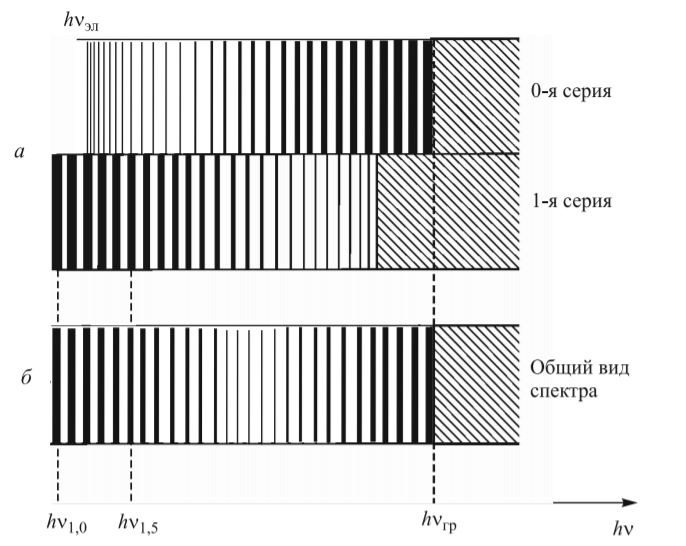
\includegraphics[scale=0.5]{йиод спекр т.png}}
\caption{Вид спектра в глазок установки}
\label{fig:image}
\end{figure}
    \item
    Cнимем следующие показания: 
\begin{enumerate}
    \item линия $h\nu_{10}$ - одна из самых длинноволновых линий спектра ($\Rightarrow$ одна из самых маленьких частот/энергий)
    \item линия $h\nu_{15}$ - шестая по счету от $h\nu_{10}$
    \item линия $h\nu_{\text{гр}}$ - на границе спектра поглощения (самая коротковолновая линия $\Rightarrow$ самая большая частота и энергия)
\end{enumerate}
По полученным значениям длин волн рассчитаем энергии соответствующих переходов по формуле
$E = \frac{hc}{\lambda}, h = 4.135 \cdot 10^{-15} \text{эВ}, \sigmaE = E \cdot \frac{\sigma \lambda}{\lambda}$. Так как эксперимент был неточным из-за засветки и слишком маленького расстояния между спектральными линиями (по сравнению с предыдущим опытом), то при расчетах погрешность измерения положения спектральных линий увеличена до $\sigma x = 20^{\circ}$ для 10 и 15, до $\sigma x = 50^{\circ}$ для групповой - там было совсем неточно.

\begin{table}[h!]
\centering
\begin{tabular}{|c|c|c|c|c|c|}
\hline
 & $x^{\circ}$ & $\lambda, A$ & $\sigma \lambda, A$ & $E, \text{эВ}$ &  $\sigma E$, эВ\\ \hline
10 & 2682 & 6250 & 50 & 1,98 & 0,02 \\ \hline
15 & 2578 & 6010 & 40 & 2,06 & 0,02 \\ \hline
гр & 1192 & 4352 & 35 & 2,85 & 0,03 \\ \hline
\end{tabular}
\end{table}


\end{itemize}


\begin{figure}[h!]
\centering
\center{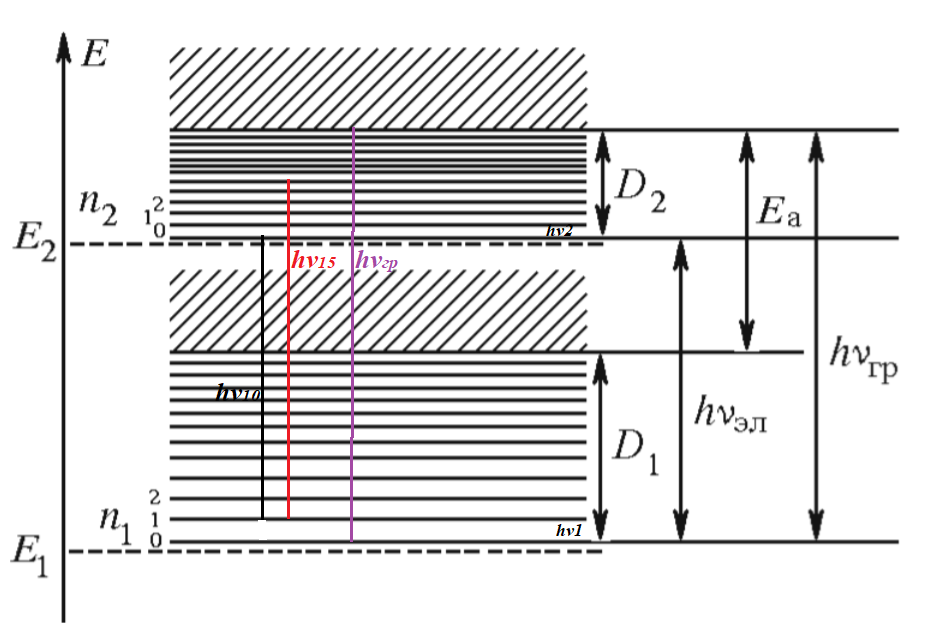
\includegraphics[scale=0.5]{уровни обработка.png}}
\caption{Уровни энергии молекулы йода. $E_1$ - основное состояние, $E_2$ - возбужденное состояние}
\label{fig:image}
\end{figure}

\begin{itemize}
\item 
Формула для n-го колебательного уровня энергии в электронном состоянии $E_i = h \nu_i$ при условии пренебрежения ангармонизмом (допустимо при малых n):
\begin{equation*}
    E_{i_n} = E_i + h \nu_i (n + \frac{1}{2})
\end{equation*}

Поэтому для расчета энергии колебательного кванта в возбужденном состоянии (2) можно воспользоваться формулой
\begin{equation*}
    h\nu_2 = \frac{h\nu_{15} - h\nu_{10}}{5}, \sigma (h\nu_2) = \frac{\sqrt{\sigma^2 (h\nu_{15}) + \sigma^2 (h\nu_{10}})}{5} \Rightarrow \boxed{h\nu_2 = (0.016 \pm 0.005) \text{эВ}}
\end{equation*}

\item 
Энергия электронного перехода (с учетом $h\nu_1 = 0.027\text{эВ}$)
\begin{equation*}
    h\nu_{\text{эл}} = h \nu_{10} - h \nu_{2} (0 + \frac{1}{2}) + h \nu_{1} (1 + \frac{1}{2}), \sigma( h\nu_{\text{эл}}) = \sqrt{\sigma^2 (h\nu_{10}) + \frac{\sigma^2 (h\nu_{2})}{4} } \Rightarrow \boxed {h\nu_{\text{эл}} = (2.01 \pm 0.02) \text{эВ}}
\end{equation*}

\item Энергия диссоциации молекулы йода в основном состоянии (с учетом энергии возбуждения $E_a = 0.94$эВ)
\begin{equation*}
    D_1 = h \nu_{\text{гр}} - E_a, \sigma D_1 = \sigma (h \nu_{\text{гр}}) \Rightarrow \boxed{D_1 = (1.91 \pm 0.03) \text{эВ}}
\end{equation*}


\item Энергия диссоциации молекулы йода в возбужденном состоянии
\begin{equation*}
    D_2 = h\nu_{\text{гр}} - h\nu_{\text{эл}}, \sigma D_2 = \sqrt{\sigma^2 ({h\nu_{\text{гр}}}) + \sigma^2 (h\nu_{\text{эл}})} \Rightarrow \boxed{ D_2 = (0.84 \pm 0.04) \text{эВ}}
\end{equation*}
\item Оценим достоверность полученных результатов. Так как экспериментально полученное $h\nu_{\text{гр}} = 2.85$эВ выше теоретического значения 2.44эВ, то  расчитанные энергии диссоциации тоже завышены по сравнению с теоретическими ($D_1 = 1.5425$эВ, $D_2 = 0.69$эВ). Такое расхождение проиошло из-за очень нечеткой границы схождения спектра молекулы йода и усталости экспериментатора к концу проведения лабораторной работы. 


\end{itemize}

\section*{Выводы}
\begin{enumerate}
    \item В ходе эксперимента по изучению спектра атома водорода проверено выполнение обобщенной формулы Бальмера для трех линий серии Бальмера, лежащих в видимой области.\newline
    Экспериментально получена постоянная Ридберга $\bar R = (109500 \pm 300) \text{см}^{-1}$, совпадающая с теоретическим значением в пределах погрешности.
    \item В ходе эксперимента по изучению спектра молекулы йода были расчитаны энергии диссоциации молекулы в основном и возбужденном состоянии. Полученные значения близки к теоретическим, однако несколько завышены предположительно из-за ошибки экспериментатора и неточности методики эксперимента.
\end{enumerate}
\end{document}